\documentclass[kravspec/krav.tex]{subfiles}

\begin{document}

\clearpage
\section{Kommunikationsmodul}
\begin{figure}[H]
    \centering
    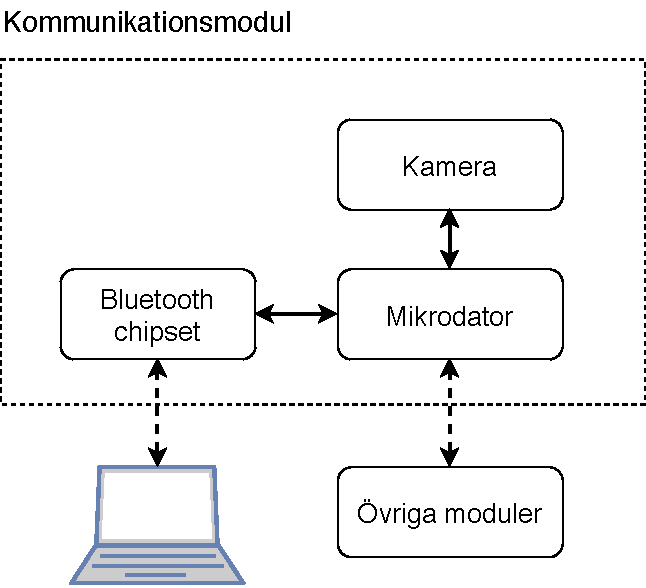
\includegraphics[width=0.6\linewidth]{kravspec/figures/kommunikationsmodul.pdf}
    \caption{Kommunikationsmodul}
    \label{fig:kommunikationsmodul}
\end{figure}

\subsection{Beskrivning}
Kommunikationsmodulen består av en mikrodator, ett bluetooth chipset samt en
kamera. Kommunikationsmodulen är huvudorganet i systemet och agerar som
dirigent. Modulen kommunicerar med alla andra moduler samt datorn och kopplar
samman dem.

\subsection{Gränssnitt}
Dess uppgift består av bland annat bildbearbetning, dirigering av information
till andra moduler samt kommunikation med en dator. Till datorn skickas
positionen på bilen, avlagd sträcka, avstånd till vägkant/hinder etc. Dessutom
används datorn som kontroller vid manuell körning av bilen.

\subsection{Krav}
\begin{reqlist}
    \req{Kommunikationsmodulen skall...}
    \req{}
\end{reqlist}

\clearpage
\section{Styrmodul}
\begin{figure}[h]
    \centering
    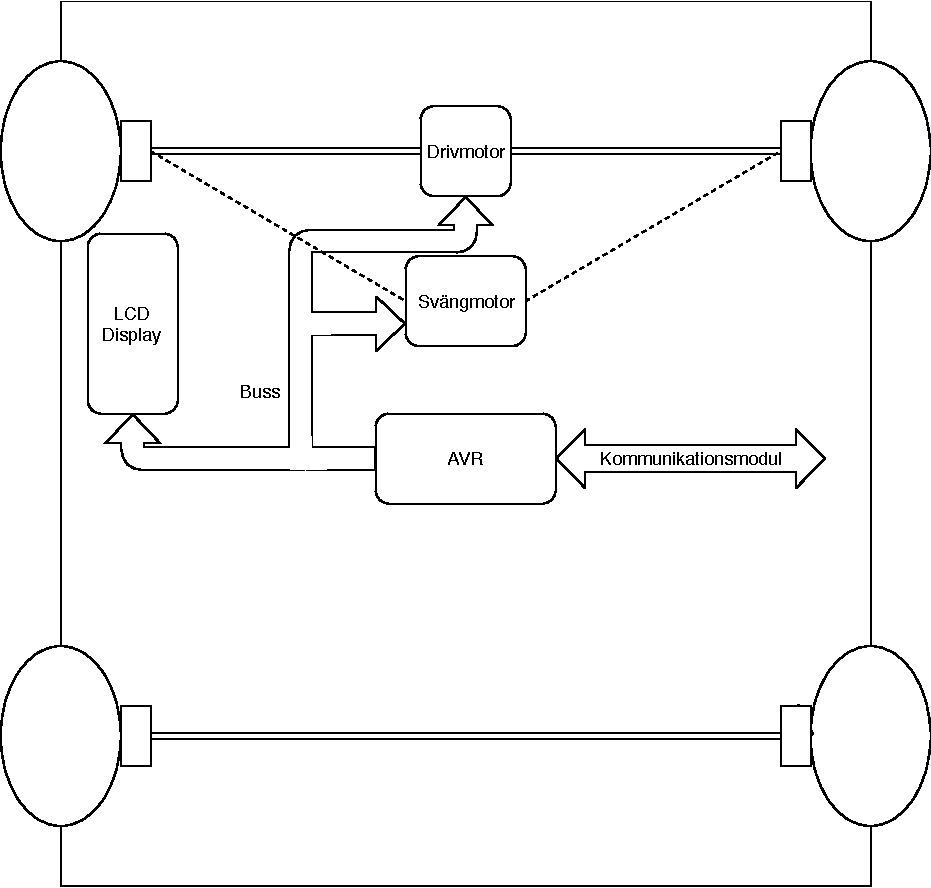
\includegraphics[width=0.6\linewidth]{kravspec/figures/styrmodul.pdf}
    \caption{Styrmodul}
    \label{fig:styrmodul}
\end{figure}

\subsection{Beskrivning}
Styrmodulen har som uppgift att ställa hjulen i rätt position samt att Taxin
håller rätt hastighet. Styrmodulen är kopplad till kommunikationsmodulen ifrån
den får information om hur Taxins hjul ska bete sig.

\subsection{Gränssnitt}
Styrmodulen består av en kontroller, en drivmotor och en styrmotor. Styrmotorns
uppgift är att hjulen ska vara i rätt position så att Taxin åker i önskad
riktning. Drivmotorn är den motor som gör att bilen får en hastighet. Alltså
köra fram eller bakåt.

\subsection{Krav}
\begin{reqlist}
    \req{Styrsystemet ska vara så exakt att Taxin kan följa banan.}
    \req{}
\end{reqlist}

\clearpage
\section{Sensormodul}
\begin{figure}[h]
    \centering
    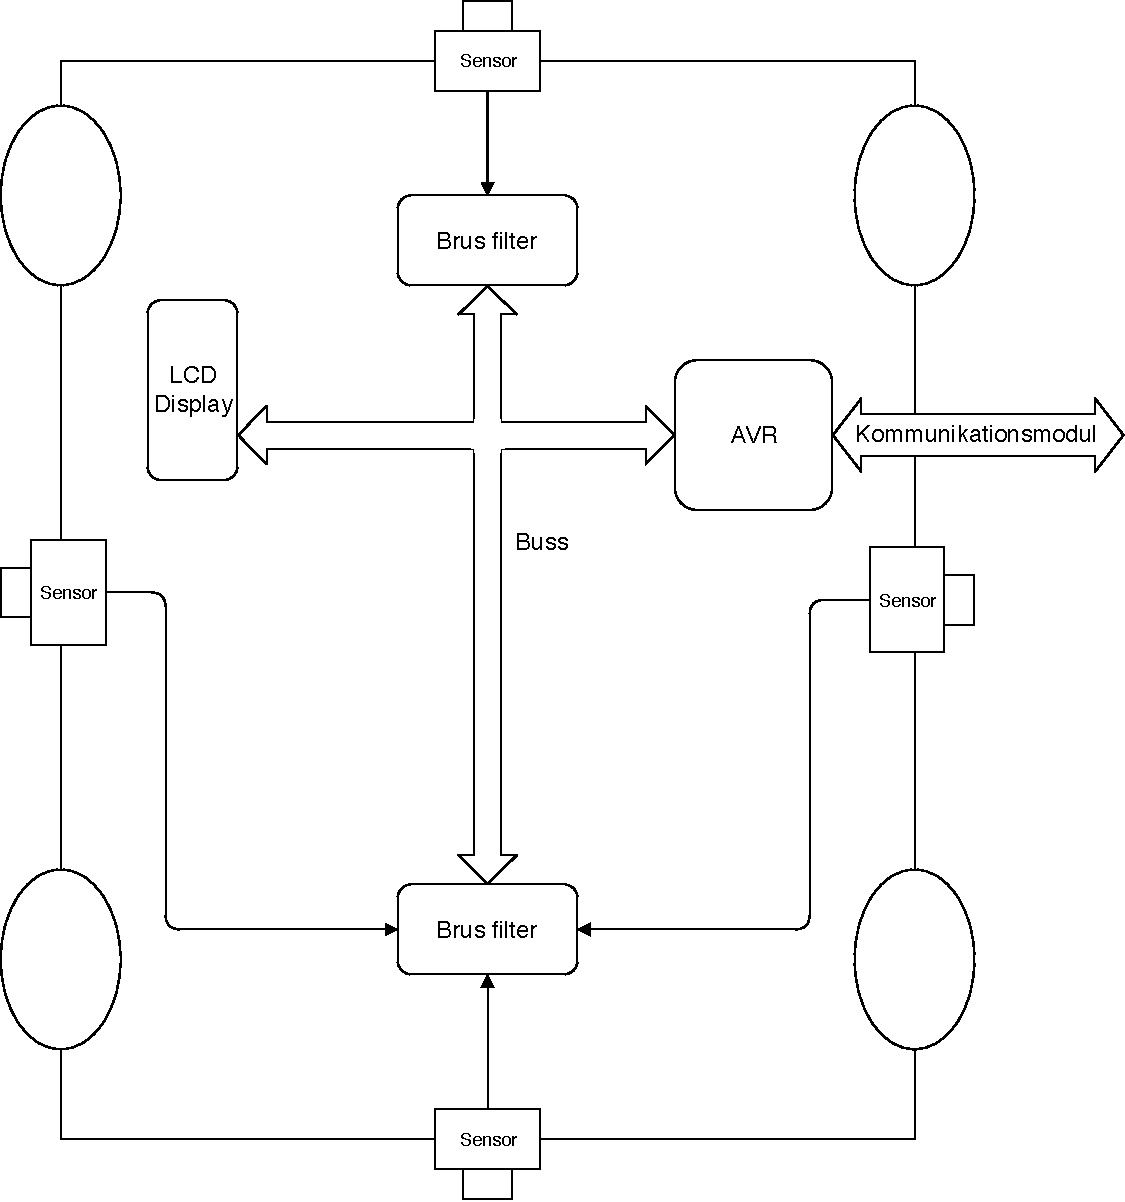
\includegraphics[width=0.6\linewidth]{kravspec/figures/sensormodul.pdf}
    \caption{Sensormodul}
    \label{fig:sensormodul}
\end{figure}

\subsection{Beskrivning}
Sensormodulen ska bestå av enhetens alla sensorer utöver kameran och en
mikrodator. Sensorerna skall väljas utefter de krav som behöver uppfyllas.
Mikrodatorns uppgift är att vidarebefodra sensorernas information till
kontrollmodulen via ett specificerat gränssnitt. Eventuellt kan kontrollmodulen
behöva utföra behandling av information innan den skickas till kontrollmodulen.

\subsection{Gränssnitt}
Sensormodulen ska bestå av alla de sensorer som Taxin ska använda. De ska vara kopplade till en kontroller som behandlar datan och skickar den till vidare till kommunikationsmodulen.
\subsection{Krav på styrmodul}
\begin{reqlist}
    \req{Sensormodulen ska kunna behandla indata från sensorer och sammanställa dessa till en bestämt gränssnitt.}
    \req{}
\end{reqlist}

\end{document}
